
\section{Evaluation}\label{sec:evaluation}

In evaluating the real-time efficacy of the DeepPicar, the methodology is consistent across all 
experiments. The performance of the platform is measured over a set of 1001 video frames that are 
each individually fed to the model. The processing time for the first frame is omitted as, due to 
cache warmup, it is uncharacteristically high and doesn't accurately represent the Picar's capabilities. 
A WCET of 50 ms, or 20 Hz, is used as a baseline to assess the platform's ability to complete all 
necessary real-time operations in a timely manner.

\subsection{Real-Time Operations}
We seek to determine if the DeepPicar is capable of consistently executing all necessary functions 
before their given deadlines. In the case of our platform, it has to process every given frame and get 
the predicted angles from the model within a WCET of 50 ms. In order to determine if this was achievable, 
we tested the platform by running a single model that utilized all 4 cpu cores and measured the time it 
took for each frame to be processed. The performance of the DeepPicar can be seen in Figure 6. We found 
that DeepPicar was able to completely process the vast majority of the provided frames within 50 ms, and 
was unable to do so for very few frames.

\begin{figure}[h]
  \centering
  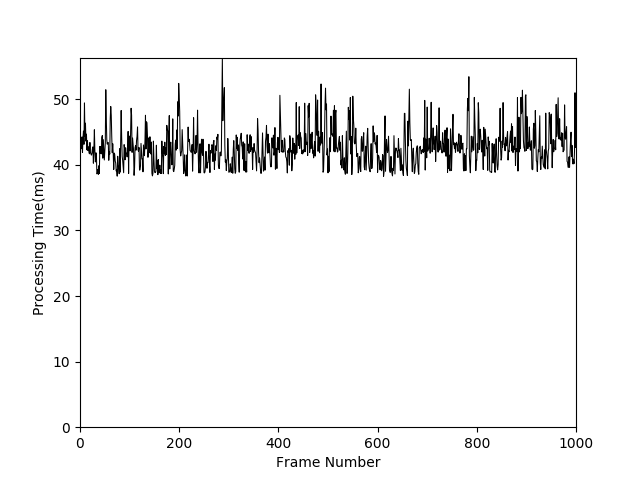
\includegraphics[width=.5\textwidth]{Total_Processing_Time}
  \caption{ Real-time performance of the Raspberry Pi 3 in processing 1000 frames.}
\end{figure}

In our platform, three main real-time tasks are performed during autonomous operation. In order, these 
operations are: (1) capturing and reading the input frame from the designated camera or video stream, 
(2) preprocessing the acquired frame so that it is compatible with the DNN, and (3) feeding the frame 
to, and getting the angle prediction from, the model. We aim to determine which operation(s), if any, 
require the most time to be performed.

\begin{table}[h]
  \centering
  \begin{tabular} {| l | l | l | l | l |}
    \hline
    \textbf{operation} & \textbf{mean} & \textbf{max} & \textbf{99pct} & \textbf{stdev} \\ \hline 
    Frame Capture & 2.28 & 4.94 & 4.54  & 0.52\\ \hline
    Preprocessing & 3.09 & 4.60 & 3.31 & 0.10 \\ \hline
    Angle Prediction & 37.30 & 51.03 & 45.48 & 2.75 \\  \hline
    Total Time & 42.67 & 56.37 & 50.70 & 2.80 \\
    \hline
  \end{tabular}
  \caption{Real-time performance of DeepPicar for each autonomous vehicle operation performed.}
\end{table}

In order to determine which operation(s) take the longest to execute, we measured the time it 
took for each step to be completed. For this experiment, all four of the Pi's cpu cores were utilized, 
and only one model was run. As is shown in Table II, the angle prediction operation consumes the 
majority of the processing for each frame. Furthermore, the time it takes for the operation to 
complete is volatile, and can range anywhere between 30 ms and 50 ms for any particular frame. On the 
other hand, both the frame capture and preprocessing operations take substantially less time 
and are relatively more consistent in their times, at 2 ms and 3 ms, respectively. 

\subsection{Multicore Performance}
It may not always be the case that all four cores of the Raspberry Pi 3's Cortex A-53 CPU can be used 
solely for the purpose of operating an autonomous vehicle. Thus, we test how the number of cores 
utilized for real-time operations affects the Pi's overall ability to function as an autonomous 
vehicle platform.

\begin{table}[h]
  \centering
  \begin{tabular} {| l | l | l | l | l | l | l | l | l | l |}
    \hline
    \textbf{num cores} & \textbf{mean} & \textbf{max} & \textbf{99pct} & \textbf{stdev} \\ \hline 
    1 & 61.96 & 66.00 & 63.31 & 0.51\\ \hline
    2 & 50.49 & 71.55 & 70.03 & 4.18 \\ \hline
    3 & 48.11 & 72.22 & 58.45 & 2.80 \\ \hline
    4 & 42.67 & 56.37 & 50.70 & 2.80 \\
    \hline
  \end{tabular}
  \caption{Real-time performance of DeepPicar depending on the number of cores used.}
\end{table}

The performance of the DeepPicar is summarized in Table III. The DeepPicar performed better, on average, 
when it utilized more cores. With 4 cores, it was able to meet the vast majority of its deadlines, doing 
so in almost 99\% of the input frames. The platform performed the worst when using only 1 core, 
as it was unable to meet any of its deadlines.  On average, using 3 cores instead of 2 only had a 
performance increase of approximately 2 ms, so the addition of one core in that specific case offers 
relatively little improvement. One important observation is that the performance was more consistent 
when only 1 core was used. As a result, the use of multiple cores is very beneficial in terms of 
reducing the time it takes to complete inference operations, but may result in times that are more 
volatile.

\subsection{Multimodel Performance}
We also test the capability of the DeepPicar to run multiple models at the same time, and whether each 
model can successfully perform within the given deadline. Specifically, the platform is tested in the 
cases of running 2 and 4 models simultaneously. For each case, all models are allocated an equal number 
of cores. That is, 2 models are given 2 cores each and 4 models are given 1 core each.

\begin{table*}
  \centering
  \begin{tabular} {| l | l | l | l | l | l | l | l | l |}
  \hline
  \textbf{num models} & \textbf{cores} & \textbf{mean} & \textbf{L1 refs} & \textbf{L1 
    misses} & \textbf{L1 miss \%} & \textbf{L2 refs} & \textbf{L2 misses} & \textbf{L2 miss \%} \\ \hline
  1 & 0,1 & 51.35 & 3.04E+10 & 4.78E+08 & 1.58 & 3.31E+09 & 3.68E+08 & 11.12\\ \hline
  2 & 0,1 & 58.03 & 3.04E+10 & 4.91E+08 & 1.61 & 3.91E+09 & 4.26E+08 & 10.88 \\ \hline
  2 & 2,3 & 56.40 & 3.04E+10 & 4.80E+08 & 1.58 & 3.88E+09 & 4.21E+08 & 10.87 \\ \hline
  \end{tabular}
  \caption{Real-time performance of the DeepPicar when 2 models are running simultaneously.}
\end{table*}

The results for the 2 model test are outlined in Table IV, and the 4 model test is summarized in Table 
V. In the the 2 model test, both of the models showed average inference time increases of around 5-7 
ms, $\sim$10\%, when compared to a baseline of 1 model running on two cores. The difference was even 
greater in the 4 model test, as each model displayed an average inference time increase of 
approximately 15 ms, $\sim$30\%, when compared to a single model running on 1 core.

The increase in inference times, however, was not the result of increased cache misses due to 
additional accesses. For all models, the number of L1 misses was always $\sim$1.6\% of all 
references. In the 2 model test, L2 cache misses remained at $\sim$11\% of all references, and each 
model in the 4 model test missed $\sim$13\% of all L2 references.

\begin{table*}
  \centering
  \begin{tabular} {| l | l | l | l | l | l | l | l | l |}
  \hline
  \textbf{num models} & \textbf{core} & \textbf{mean} & \textbf{L1 refs} & \textbf{L1 
    misses} & \textbf{L1 miss \%} & \textbf{L2 refs} & \textbf{L2 misses} & \textbf{L2 miss \%} \\ \hline
    1 & 0 & 62.48 & 2.78E+10 & 4.36E+08 & 1.57 & 2.83E+09 & 3.59E+08 & 12.68 \\ \hline
    4 & 0 & 77.90 & 2.79E+10 & 4.53E+08 & 1.63 & 3.36E+09 & 4.43E+08 & 13.19 \\ \hline
    4 & 1 & 78.89 & 2.79E+10 & 4.64E+08 & 1.67 & 3.42E+09 & 4.38E+08 & 12.82 \\ \hline
    4 & 2 & 77.81 & 2.78E+10 & 4.45E+08 & 1.60 & 3.45E+09 & 4.41E+08 & 12.77 \\ \hline
    4 & 3 & 77.87 & 2.79E+10 & 4.45E+08 & 1.60 & 3.41E+09 & 4.39E+08 & 12.88 \\ \hline
  \end{tabular}
  \caption{Real-time performance of the DeepPicar when 4 models are running simultaneously.}
\end{table*}

In all multimodel tests, it was found that a greater number of models run simultaneously resulted in 
interference that led to a noticable increase in the average inferencing time that wasn't 
attributable to a change in cache misses. Instead, the overall time increases can most likely be 
traced to an increase in cache latency. Even if the models had a consistent number of cache hits, it 
is highly probable that the contention for the cache increased the access time for each model, 
consequently increasing the time it took for the models to execute their operations.

In terms of real-time performance under a WCET of 50 ms, the DeepPicar was unsatisfactory in all 
multimodel tests. On average, the 2 model test saw models miss their deadline by 6-8 ms, and the 4 
model test was worse as each model went over their deadlines by 27-29 ms. As a result, it can be 
ascertained that, if a WCET of 50 ms is required, DeepPicar would not be able to perform as necessary.

\subsection{Benchmark Performance}
In order to determine how cache misses affects the performance of the DeepPicar, we test its ability by 
running synthetic benchmarks concurrently with the model. In each experiment, we run a single model on a 
number of cores, and a synthetic benchmark on the remaining idle cores. The results of each test can be 
seen in Table VII.

\begin{table}[h]
\centering
  \begin{tabular} {| l | l | l | l | l | l |}
  \hline
  \textbf{num cores} & 1 & 2 & 3 \\ \hline
  \textbf{mean} & 562.33 & 391.98 & 98.05 \\ \hline
  \textbf{L1 refs} & 3.16E+10 & 3.17E+10 & 3.06E+10 \\ \hline
  \textbf{L1 misses} & 5.41E+08 & 5.35E+08 & 4.98E+08 \\ \hline
  \textbf{L1 miss \%} & 1.71 & 1.69 & 1.62 \\ \hline
  \textbf{L2 refs} & 3.49E+09 & 3.23E+09 & 3.21E+09 \\ \hline
  \textbf{L2 misses} & 8.05E+08 & 7.54E+08 & 4.98E+08 \\ \hline
  \textbf{L2 miss \%} & 23.05 & 23.37 & 15.51 \\ 
  \hline
  \end{tabular}
  \caption{Real-time performance of the DeepPicar when benchmarks are run concurrently with the model.}
\end{table}

The presence of the benchmark(s) had a noticable effect on the DeepPicar, with all tests showing 
increases in inferencing operations. The least change happened when the model was run on 3 cores, and a 
single benchmark was run on the final core. Even with a slight increase in the number of L2 cache 
misses, inferencing was able to be completed in under 100 ms. The other tests, however, showed dramatic 
changes when the model was run on 1 and 2 cores. In both instances, L2 misses rise to $\sim$23\% of all 
references. The additional benchmark in the 1 core test was even more detrimental as the average 
inferencing time was at least 150 ms longer than when the model used 2 cores. 

With the introduction of synthetic benchmarks, the DeepPicar failed to comply with the 50 ms WCET across 
all tests run. Even in the best case, inferencing operations take twice as long as the deadline to 
complete. As a result, if benchmarks were required to run during autonomous operation, the DeepPicar 
wouldn't be capable of meeting its deadlines.

\subsection{Summary}
We found that the DeepPicar is capable of successfully completing all necessary inferencing 
operations within a given deadline of 50 ms. Between these operations, it was discovered that the 
angle prediction time of the model was the dominating step in the processing time of a single frame. 
The other operations were found to execute in very little time, with either one taking 5 ms at most.

When running a single model, DeepPicar performed the best when it used all 4 cpu cores, as it was 
able to process a frame in 43 ms on average. This feat can still be accomplished when running a 
single model on 3 cpu cores, and is also possible when using 2 cores. The only time in which the Pi 
can't run a single model under 50 ms is when only 1 core is used. This was also the case when 
multiple models were run concurrently as no models were able to consistently complete inference 
operations in under 50 ms.

However, the DeepPicar was shown to be capable of handling other potential WCETs. If given a larger 
deadline, the capabilities of DeepPicar as an autonomous vehicle platform would be greatly increased. 
For example, if tested with a deadline of 66.67 ms, or 15 fps, the platform would have passed several 
of the experiments performed. In actuality, the DeepPicar would have only been unsatisfactory in the 
4 model test where it would have missed the deadlines by $\sim$10 ms, and the benchmark tests, where 
it would still miss by $\sim$33 ms at best.

\subsection{Performance Requirements}
In the utilization of the Raspberry Pi 3 in our platform, there are a few factors that need to be 
considered and/or enforced in order to guarantee that the Pi is able to consistently perform at a 
desired level. Specifically, these issues all have the potential to negatively affect the cpu clock 
speed/frequency, which would result in decreased performance. While, in the above experiments, the cpu 
operated at a preferred clock speed of 1.2 GHz, it is entirely possible for the cpu to operate at a 
lower frequency if the following problems are not taken into account.

The most notable issue that can affect the cpu clock speed is that of the power supplied to the 
Raspberry Pi. In essence, it is necessary that the Pi be supplied with 2 Amps, as any less could 
hinder the Pi's ability to maintain a 1.2 GHz frequency. In experiments conducted with a power supply that 
only provided 1 Amp, the Pi was unable to sustain a 1.2 GHz clock speed and, instead, fluctuated 
between operating at 600 MHz and 1.2 GHz. As a result, it is necessary, or at least highly 
recommended, that the power supply used for the Raspberry Pi 3 be capable of outputting 2 Amps, 
otherwise optimal performance isn't guaranteed.

Another factor that can affect clock speed is that of the cpu's temperature. Some model operations can 
be computationally intensive, thus it is possible for the temperature of the cpu to become relatively 
high. This can be especially problematic in situations where multiple models are running 
simultaneously on the Pi. Consequently, thermal throttling may be used to decrease the clock 
speed so that the cpu temperature stays at a safe level. Thus the Raspberry Pi may not be suited 
for prolonged use, especially in cases where the workload is relatively larger, such as running multiple 
models. Rather, the Pi seems to be better suited for running in set periods, after which it is turned 
off or made idle so that the cpu is allowed time to cool down.
